\documentclass[11pt]{article}
% Revised September 22, 2026.
% PDF reproduction: compile to the corresponding public/pdfs path, then run
% python scripts/stamp-pdf-revisions.py in the website checkout (pypdf, reportlab).
% This adds only a first-page margin date; it does not reflow mathematical content.

\usepackage[margin=1in]{geometry}
\usepackage[T1]{fontenc}
\usepackage[utf8]{inputenc}
\usepackage{mathpazo}
\usepackage{microtype}
\usepackage{amsmath,amssymb,amsthm,mathtools}
\usepackage{xcolor}
\usepackage{tikz}
\usetikzlibrary{arrows.meta,positioning,calc,decorations.pathreplacing}
\usepackage[colorlinks=true,linkcolor=blue!60!black,citecolor=blue!60!black,urlcolor=blue!60!black]{hyperref}

\title{\vspace{-2em}{\Huge\bfseries Divisibility of Separated Polynomials}\\[0.45em]
{\Large Free Modules, Diagonal Reduction, and Applications}}
\author{Henry Shin}
\date{}

\theoremstyle{plain}
\newtheorem{theorem}{Theorem}[section]
\newtheorem{proposition}[theorem]{Proposition}
\newtheorem{lemma}[theorem]{Lemma}
\newtheorem{corollary}[theorem]{Corollary}

\theoremstyle{definition}
\newtheorem{definition}[theorem]{Definition}
\newtheorem{example}[theorem]{Example}

\theoremstyle{remark}
\newtheorem{remark}[theorem]{Remark}

\newcommand{\kk}{k}
\newcommand{\U}{U}
\newcommand{\V}{V}
\newcommand{\TT}{T}
\newcommand{\ZZ}{Z}
\newcommand{\A}{\mathbb A}
\newcommand{\calB}{\mathcal B}
\newcommand{\ol}[1]{\overline{#1}}

\begin{document}

\maketitle

\begin{abstract}
Let \(k\) be a field and let \(f,g,p,q\in k[t]\), with \(f\) and \(g\) nonconstant. We prove that
\[
    f(x)-g(y)\mid p(x)-q(y) \quad \text{in } k[x,y]
\]
if and only if there is a single polynomial \(s\in k[t]\) such that
\[
    p=s\circ f, \qquad q=s\circ g.
\]
The proof uses the fact that \(k[x]\) is a free \(k[f]\)-module with basis
\(1,x,\dots,x^{\deg f-1}\), and then applies this independently in the two variables. The resulting residue rectangle in \(k[x,y]\) turns the divisibility hypothesis into coefficient identities in \(k[U,V]\). The final step is the diagonal specialization \(U=V\), equivalently reduction modulo \(U-V\). We also include an explicit algorithm for extracting the common outer polynomial and an application to a symmetric functional equation whose branches come from the fibers of \(t^3+t\).
\end{abstract}

\section{Statement and first comments}

Separated polynomials, namely polynomials of the form \(p(x)-q(y)\), occur naturally in factorization problems, fiber products of polynomial maps, and functional equations with conjugate branches. The following theorem says that divisibility by another separated polynomial \(f(x)-g(y)\) is rigid: it occurs exactly when \(p\) and \(q\) both descend from the same one-variable polynomial on the common value of \(f\) and \(g\).

\begin{theorem}[Separated divisibility criterion]\label{thm:main}
Let \(k\) be a field, and let
\[
    f,g,p,q\in k[t],
    \qquad \deg f>0,
    \qquad \deg g>0.
\]
Then
\[
    f(x)-g(y)\mid p(x)-q(y)
    \qquad \text{in } k[x,y]
\]
if and only if there exists \(s\in k[t]\) such that
\[
    p(t)=s(f(t)),
    \qquad
    q(t)=s(g(t)).
\]
\end{theorem}

The reverse implication is immediate. If \(p=s\circ f\) and \(q=s\circ g\), then
\[
    p(x)-q(y)=s(f(x))-s(g(y)).
\]
For every polynomial \(s\), the difference \(s(\U)-s(\V)\) is divisible by \(\U-\V\) in \(k[\U,\V]\), so after substituting
\[
    \U=f(x), \qquad \V=g(y),
\]
we get
\[
    f(x)-g(y)
    \mid
    s(f(x))-s(g(y))
    =p(x)-q(y).
\]
The forward implication is the substantial part.

\section{The one-variable free-module expansion}

We first isolate the basic one-variable fact. It is useful to state it over a general integral domain, because in the two-variable proof the coefficient ring will temporarily be \(k[y]\) or \(k[U]\).

\begin{lemma}[One-variable residue expansion]\label{lem:one-variable}
Let \(R\) be an integral domain, and let
\[
    F(t)=\lambda t^d+\alpha_{d-1}t^{d-1}+\cdots+\alpha_0\in R[t],
\]
where \(d>0\) and \(\lambda\in R^\times\). Then
\[
    R[t]
    =
    \bigoplus_{i=0}^{d-1} R[F]t^i.
\]
Equivalently, every \(H(t)\in R[t]\) has a unique expression
\[
    H(t)=\sum_{i=0}^{d-1} A_i(F(t))t^i,
    \qquad A_i\in R[T].
\]
\end{lemma}

\begin{proof}
Since \(\lambda\) is a unit in \(R\), we may solve for \(t^d\):
\[
    t^d
    =
    \lambda^{-1}F(t)
    -
    \lambda^{-1}\sum_{r=0}^{d-1}\alpha_r t^r.
\]
This identity reduces the power \(t^d\) to an \(R[F]\)-linear combination of
\[
    1,t,\dots,t^{d-1}.
\]
Multiplying by powers of \(t\) and arguing by induction, every monomial \(t^N\) belongs to
\[
    \sum_{i=0}^{d-1} R[F]t^i.
\]
Therefore the displayed sum spans \(R[t]\).

For uniqueness, suppose
\[
    \sum_{i=0}^{d-1} A_i(F(t))t^i=0,
    \qquad A_i\in R[T].
\]
Assume some \(A_i\) is nonzero. For each nonzero \(A_i\), write
\[
    A_i(T)=a_i T^{e_i}+\text{lower powers of }T,
    \qquad a_i\neq 0.
\]
Since \(R\) is an integral domain and \(\lambda\) is a unit, the leading term of \(A_i(F(t))t^i\) has degree
\[
    d e_i+i.
\]
For distinct \(i\in\{0,\dots,d-1\}\), the integers \(d e_i+i\) lie in distinct congruence classes modulo \(d\). Hence among the nonzero summands there is a unique summand of largest \(t\)-degree. Its leading term cannot cancel with anything else. This contradicts the equality to zero.

Thus all \(A_i\) vanish, and the expansion is unique.
\end{proof}

\begin{remark}[No monicity needed]
The polynomial \(F\) need not be monic. We only need its leading coefficient to be a unit. In the main theorem the coefficient ring is a field, so every nonzero leading coefficient is automatically a unit.
\end{remark}

\begin{corollary}\label{cor:univariate-kf}
Let \(k\) be a field and let \(f\in k[t]\) have degree \(n>0\). Then
\[
    k[x]
    =
    \bigoplus_{i=0}^{n-1} k[f(x)]x^i.
\]
In particular, every \(p(x)\in k[x]\) has a unique expression
\[
    p(x)=\sum_{i=0}^{n-1} a_i(f(x))x^i,
    \qquad a_i\in k[T].
\]
\end{corollary}

\section{The two-variable residue rectangle}

Set
\[
    n=\deg f,
    \qquad
    m=\deg g.
\]
The next proposition is the structural heart of the proof.

\begin{proposition}[Two-variable residue expansion]\label{prop:bivariate-expansion}
Let \(f,g\in k[t]\) have degrees \(n>0\) and \(m>0\), respectively. Then every polynomial \(H(x,y)\in k[x,y]\) admits a unique expression
\[
    H(x,y)
    =
    \sum_{0\leq i<n,\;0\leq j<m}
    C_{ij}(f(x),g(y))x^i y^j,
\]
where
\[
    C_{ij}(\U,\V)\in k[\U,\V].
\]
Equivalently,
\[
    k[x,y]
    =
    \bigoplus_{0\leq i<n,\;0\leq j<m}
    k[f(x),g(y)]x^i y^j.
\]
Thus \(k[x,y]\) is a free \(k[f(x),g(y)]\)-module of rank \(nm\), with basis
\[
    \calB=
    \{x^i y^j:0\leq i<n,
    \;0\leq j<m\}.
\]
\end{proposition}

\begin{proof}
We first prove existence. Regard \(k[x,y]\) as \(k[y][x]\). Applying Lemma~\ref{lem:one-variable} with coefficient ring \(R=k[y]\) and polynomial \(f(x)\), we can write
\[
    H(x,y)
    =
    \sum_{i=0}^{n-1} A_i(f(x),y)x^i,
\]
where
\[
    A_i(\U,y)\in k[\U,y].
\]
Now fix \(i\). Regard \(A_i(\U,y)\) as a polynomial in \(y\) with coefficients in the integral domain \(k[\U]\). Applying Lemma~\ref{lem:one-variable} again, now with polynomial \(g(y)\), gives
\[
    A_i(\U,y)
    =
    \sum_{j=0}^{m-1} C_{ij}(\U,g(y))y^j,
\]
for some
\[
    C_{ij}(\U,\V)
    \in
    k[\U,\V].
\]
Substituting \(\U=f(x)\) yields the desired expression.

For uniqueness, suppose
\[
    \sum_{0\leq i<n,\;0\leq j<m}
    C_{ij}(f(x),g(y))x^i y^j=0.
\]
For each \(i\), put
\[
    B_i(\U,y)
    =
    \sum_{j=0}^{m-1} C_{ij}(\U,g(y))y^j
    \in k[\U,y].
\]
Then
\[
    \sum_{i=0}^{n-1} B_i(f(x),y)x^i=0.
\]
By Lemma~\ref{lem:one-variable}, applied over the coefficient ring \(k[y]\), each polynomial \(B_i(\U,y)\) is zero. Hence, for each \(i\),
\[
    \sum_{j=0}^{m-1} C_{ij}(\U,g(y))y^j=0
    \qquad \text{in } k[\U,y].
\]
Applying Lemma~\ref{lem:one-variable} again over the coefficient ring \(k[\U]\), we obtain
\[
    C_{ij}(\U,\V)=0
\]
for every pair \((i,j)\). This proves uniqueness.
\end{proof}

\begin{remark}[Lattice intuition]
The uniqueness says that the monomials \(x^i y^j\) with
\[
    0\leq i<n,
    \qquad
    0\leq j<m
\]
form a fundamental residue rectangle. Multiplication by powers of \(f(x)\) and \(g(y)\) moves this rectangle by degree increments of size \(n\) in the \(x\)-direction and size \(m\) in the \(y\)-direction. The formal proof above avoids choosing a monomial order, but the following picture captures the degree geometry.
\end{remark}

\begin{figure}[h]
\centering
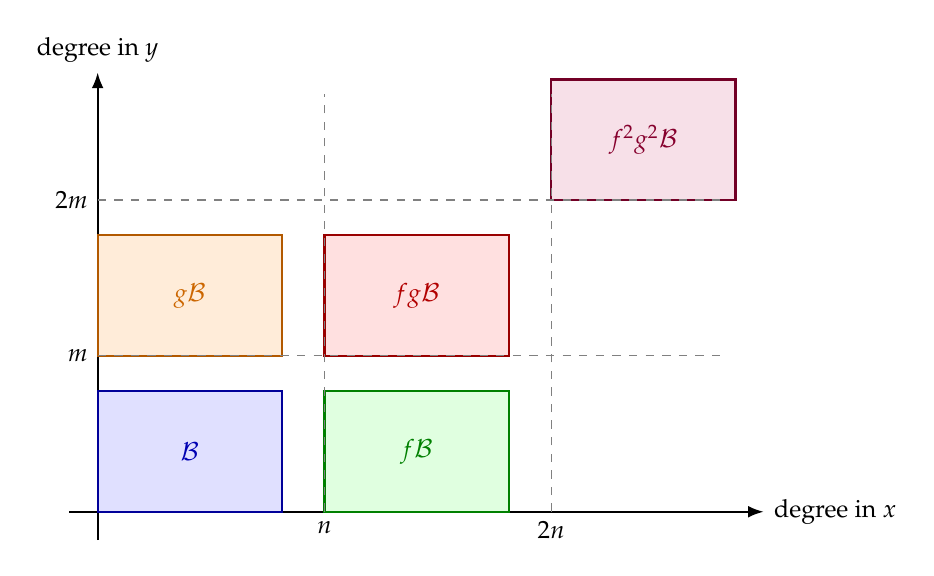
\begin{tikzpicture}[scale=0.9, every node/.style={font=\small}]
    % axes
    \draw[-{Latex[length=2mm]}, thick] (-0.4,0) -- (9.4,0) node[right] {degree in \(x\)};
    \draw[-{Latex[length=2mm]}, thick] (0,-0.4) -- (0,6.2) node[above] {degree in \(y\)};

    % fundamental rectangles
    \fill[blue!12] (0,0) rectangle (2.6,1.7);
    \draw[blue!60!black, thick] (0,0) rectangle (2.6,1.7);
    \node[blue!70!black] at (1.3,0.85) {\(\calB\)};

    \fill[green!12] (3.2,0) rectangle (5.8,1.7);
    \draw[green!50!black, thick] (3.2,0) rectangle (5.8,1.7);
    \node[green!50!black] at (4.5,0.85) {\(f\calB\)};

    \fill[orange!15] (0,2.2) rectangle (2.6,3.9);
    \draw[orange!70!black, thick] (0,2.2) rectangle (2.6,3.9);
    \node[orange!80!black] at (1.3,3.05) {\(g\calB\)};

    \fill[red!12] (3.2,2.2) rectangle (5.8,3.9);
    \draw[red!60!black, thick] (3.2,2.2) rectangle (5.8,3.9);
    \node[red!70!black] at (4.5,3.05) {\(fg\calB\)};

    \fill[purple!12] (6.4,4.4) rectangle (9.0,6.1);
    \draw[purple!60!black, thick] (6.4,4.4) rectangle (9.0,6.1);
    \node[purple!70!black] at (7.7,5.25) {\(f^2g^2\calB\)};

    % ticks / guides
    \draw[dashed, gray] (3.2,0) -- (3.2,5.9);
    \draw[dashed, gray] (6.4,0) -- (6.4,5.9);
    \draw[dashed, gray] (0,2.2) -- (8.9,2.2);
    \draw[dashed, gray] (0,4.4) -- (8.9,4.4);

    \node[below] at (3.2,0) {\(n\)};
    \node[below] at (6.4,0) {\(2n\)};
    \node[left] at (0,2.2) {\(m\)};
    \node[left] at (0,4.4) {\(2m\)};
\end{tikzpicture}
\caption{The residue rectangle \(\calB\) and some of its degree shifts under multiplication by \(f(x)\) and \(g(y)\).}
\label{fig:lattice}
\end{figure}

\begin{corollary}[Algebraic independence]\label{cor:alg-independence}
The natural homomorphism
\[
    k[\U,\V]
    \longrightarrow
    k[x,y],
    \qquad
    \U\longmapsto f(x),
    \qquad
    \V\longmapsto g(y),
\]
is injective. Equivalently, \(f(x)\) and \(g(y)\) are algebraically independent over \(k\).
\end{corollary}

\begin{proof}
If \(C(f(x),g(y))=0\), then this is a residue expansion supported only in the \((i,j)=(0,0)\) slot. By uniqueness in Proposition~\ref{prop:bivariate-expansion}, \(C=0\).
\end{proof}

\section{Proof of the divisibility criterion}

We now prove Theorem~\ref{thm:main}.

Assume
\[
    f(x)-g(y)
    \mid
    p(x)-q(y)
    \qquad \text{in } k[x,y].
\]
Then there exists \(H(x,y)\in k[x,y]\) such that
\[
    p(x)-q(y)=(f(x)-g(y))H(x,y).
\]

By Proposition~\ref{prop:bivariate-expansion}, write
\[
    H(x,y)
    =
    \sum_{0\leq i<n,\;0\leq j<m}
    C_{ij}(f(x),g(y))x^i y^j,
\]
where \(C_{ij}\in k[\U,\V]\). Then
\[
    (f(x)-g(y))H(x,y)
    =
    \sum_{0\leq i<n,\;0\leq j<m}
    (\U-\V)C_{ij}(\U,\V)\big|_{\U=f(x),\,\V=g(y)}x^i y^j.
\]

On the other hand, by Corollary~\ref{cor:univariate-kf}, the polynomials \(p\) and \(q\) have unique expansions
\[
    p(x)=\sum_{i=0}^{n-1} a_i(f(x))x^i,
    \qquad a_i\in k[\U],
\]
and
\[
    q(y)=\sum_{j=0}^{m-1} b_j(g(y))y^j,
    \qquad b_j\in k[\V].
\]
Therefore the two-variable residue expansion of \(p(x)-q(y)\) is
\[
    p(x)-q(y)
    =
    a_0(f(x))-b_0(g(y))
    +
    \sum_{i=1}^{n-1}a_i(f(x))x^i
    -
    \sum_{j=1}^{m-1}b_j(g(y))y^j.
\]

Comparing the unique coefficients in the residue rectangle gives identities in \(k[\U,\V]\):
\begin{align}
    (\U-\V)C_{ij}(\U,\V)&=0
    &&\text{for } i>0,
    \;j>0, \label{eq:interior}\\
    (\U-\V)C_{i0}(\U,\V)&=a_i(\U)
    &&\text{for } i>0, \label{eq:bottom}\\
    (\U-\V)C_{0j}(\U,\V)&=-b_j(\V)
    &&\text{for } j>0, \label{eq:left}\\
    (\U-\V)C_{00}(\U,\V)&=a_0(\U)-b_0(\V). \label{eq:origin}
\end{align}

The comparison can be visualized as follows: the right-hand side \(p(x)-q(y)\) occupies only the bottom row and the left column of the residue rectangle, while the product \((f(x)-g(y))H(x,y)\) has coefficient \((\U-\V)C_{ij}\) in every slot.

\begin{figure}[h]
\centering
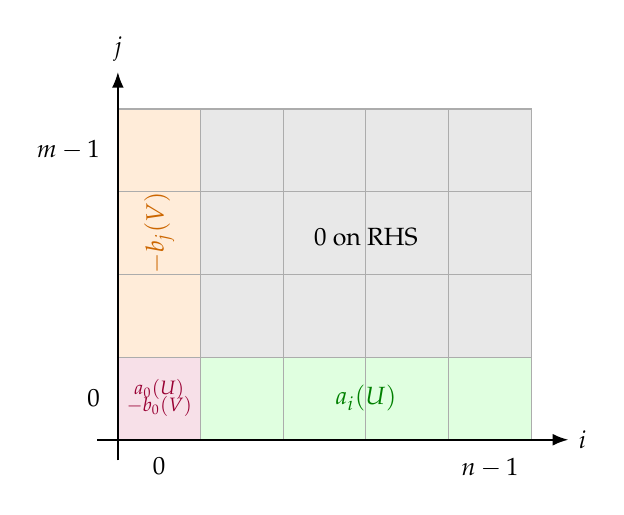
\begin{tikzpicture}[scale=1.05, every node/.style={font=\small}]
    \def\n{5}
    \def\m{4}

    % grid
    \foreach \i in {0,...,4} {
        \foreach \j in {0,...,3} {
            \draw[gray!60] (\i,\j) rectangle ++(1,1);
        }
    }

    % regions
    \fill[gray!18] (1,1) rectangle (5,4);
    \fill[green!12] (1,0) rectangle (5,1);
    \fill[orange!15] (0,1) rectangle (1,4);
    \fill[purple!12] (0,0) rectangle (1,1);

    % redraw grid
    \foreach \i in {0,...,4} {
        \foreach \j in {0,...,3} {
            \draw[gray!65] (\i,\j) rectangle ++(1,1);
        }
    }

    \node[align=center] at (3,2.45) {\(0\) on RHS};
    \node[align=center, green!50!black] at (3,0.5) {\(a_i(\U)\)};
    \node[align=center, orange!80!black, rotate=90] at (0.5,2.5) {\(-b_j(\V)\)};
    \node[align=center, purple!80!black, font=\scriptsize] at (0.5,0.5) {\(\begin{array}{c}a_0(\U)\\[-0.25em]-b_0(\V)\end{array}\)};

    \draw[-{Latex[length=2mm]}, thick] (-0.25,0) -- (5.45,0) node[right] {\(i\)};
    \draw[-{Latex[length=2mm]}, thick] (0,-0.25) -- (0,4.45) node[above] {\(j\)};

    \node[below] at (0.5,-0.1) {\(0\)};
    \node[below] at (4.5,-0.1) {\(n-1\)};
    \node[left] at (-0.1,0.5) {\(0\)};
    \node[left] at (-0.1,3.5) {\(m-1\)};
\end{tikzpicture}
\caption{The coefficient comparison in the residue rectangle.}
\label{fig:coefficient-rectangle}
\end{figure}

Since \(k[\U,\V]\) is an integral domain and \(\U-\V\neq 0\), equation~\eqref{eq:interior} gives
\[
    C_{ij}=0
    \qquad
    \text{for } i>0,
    \;j>0.
\]

Now consider the diagonal specialization map
\[
    \Delta:k[\U,\V]\longrightarrow k[\TT],
    \qquad
    \Delta(\U)=\TT,
    \qquad
    \Delta(\V)=\TT.
\]
This is the same as reducing modulo the ideal \((\U-\V)\).

Applying \(\Delta\) to equation~\eqref{eq:bottom} gives
\[
    0=a_i(\TT)
    \qquad
    \text{for } i>0.
\]
Thus
\[
    a_i=0
    \qquad
    \text{for } i>0.
\]
Then equation~\eqref{eq:bottom} also gives \(C_{i0}=0\) for \(i>0\).

Similarly, applying \(\Delta\) to equation~\eqref{eq:left} gives
\[
    0=-b_j(\TT)
    \qquad
    \text{for } j>0,
\]
so
\[
    b_j=0
    \qquad
    \text{for } j>0.
\]
Then equation~\eqref{eq:left} also gives \(C_{0j}=0\) for \(j>0\).

Finally, applying \(\Delta\) to equation~\eqref{eq:origin} gives
\[
    0=a_0(\TT)-b_0(\TT).
\]
Hence
\[
    a_0=b_0
    \qquad
    \text{in } k[\TT].
\]
Define
\[
    s(\TT)=a_0(\TT)=b_0(\TT).
\]
Since all \(a_i\) for \(i>0\) vanish, the expansion of \(p\) reduces to
\[
    p(x)=a_0(f(x))=s(f(x)).
\]
Since all \(b_j\) for \(j>0\) vanish, the expansion of \(q\) reduces to
\[
    q(y)=b_0(g(y))=s(g(y)).
\]
Replacing \(x\) and \(y\) by a single indeterminate \(t\), we get
\[
    p(t)=s(f(t)),
    \qquad
    q(t)=s(g(t)).
\]
This proves the forward implication.

For the converse, suppose \(p=s\circ f\) and \(q=s\circ g\). Write
\[
    s(T)=\sum_{\ell=0}^N c_\ell T^\ell.
\]
Then
\[
    s(\U)-s(\V)
    =
    \sum_{\ell=1}^N c_\ell(\U^\ell-\V^\ell)
    =
    (\U-\V)
    \sum_{\ell=1}^N c_\ell\sum_{r=0}^{\ell-1}\U^{\ell-1-r}\V^r.
\]
Thus \(\U-\V\mid s(\U)-s(\V)\). Substituting \(\U=f(x)\) and \(\V=g(y)\) gives
\[
    f(x)-g(y)
    \mid
    s(f(x))-s(g(y))
    =
    p(x)-q(y).
\]
The theorem follows. \qed

\section{The binomial-shift version of the diagonal step}

The diagonal map \(\Delta\) is the shortest way to express the last step of the proof. It is also useful to spell out the equivalent constructive version, because it explains exactly how terms are moved into a multiple of \(\U-\V\).

\begin{lemma}[Binomial shift]\label{lem:binomial-shift}
For every \(B(T)\in k[T]\), there is a polynomial \(Q_B(\U,\V)\in k[\U,\V]\) such that
\[
    B(\V)=B(\U)+(\V-\U)Q_B(\U,\V).
\]
More explicitly, if
\[
    B(T)=\sum_{\ell=0}^N c_\ell T^\ell,
\]
then one may take
\[
    Q_B(\U,\V)
    =
    \sum_{\ell=1}^N c_\ell
    \sum_{r=0}^{\ell-1} \V^{\ell-1-r}\U^r.
\]
\end{lemma}

\begin{proof}
Use
\[
    \V^\ell-\U^\ell
    =
    (\V-\U)\sum_{r=0}^{\ell-1}\V^{\ell-1-r}\U^r
\]
for every \(\ell\geq 1\), and sum over the terms of \(B\).
\end{proof}

Applying this lemma to \(B=b_0\), equation~\eqref{eq:origin} becomes
\[
    (\U-\V)C_{00}(\U,\V)
    =
    a_0(\U)-b_0(\U)+(\U-\V)Q_{b_0}(\U,\V).
\]
Equivalently,
\[
    (\U-\V)\bigl(C_{00}(\U,\V)-Q_{b_0}(\U,\V)\bigr)
    =
    a_0(\U)-b_0(\U).
\]
Reducing modulo \(\U-\V\), or equivalently setting \(\V=\U\), forces
\[
    a_0(\U)-b_0(\U)=0.
\]
This is precisely the same argument as the diagonal specialization, written in expanded binomial form.

\section{Algorithmic extraction of the outer polynomial}

The theorem is structural, but once the conclusion \(P=S\circ G\) is expected, the outer polynomial \(S\) can be computed directly. The following proposition gives a clean extraction method that avoids solving a large linear system for the coefficients of \(S\).

\begin{proposition}[Remainder extraction]\label{prop:algorithmic-extraction}
Let \(G(t),P(t)\in k[t]\), with \(d=\deg G>0\), and let \(Z\) be a new indeterminate. Divide \(P(t)\), as a polynomial in \(t\), by \(G(t)-Z\) over the coefficient ring \(k[Z]\):
\[
    P(t)=A(t,Z)(G(t)-Z)+R(t,Z),
    \qquad \deg_t R<d.
\]
Then
\[
    P\in k[G]
\]
if and only if the remainder \(R(t,Z)\) is independent of \(t\), i.e. \(R(t,Z)\in k[Z]\). In that case
\[
    P(t)=R(G(t))
\]
and \(R(Z)\) is the unique outer polynomial.

In particular, if it is already known that \(P(t)=S(G(t))\), then the remainder is exactly
\[
    R(t,Z)=S(Z).
\]
\end{proposition}

\begin{proof}
The division is valid in \(k[Z][t]\) because the leading coefficient of \(G(t)-Z\), viewed as a polynomial in \(t\), is the nonzero leading coefficient of \(G\), hence a unit of \(k[Z]\).

Suppose first that \(P(t)=S(G(t))\). In \(k[X,Z]\), the difference \(S(X)-S(Z)\) is divisible by \(X-Z\), so there exists \(B(X,Z)\in k[X,Z]\) such that
\[
    S(X)-S(Z)=(X-Z)B(X,Z).
\]
Substituting \(X=G(t)\) gives
\[
    P(t)=S(G(t))=(G(t)-Z)B(G(t),Z)+S(Z).
\]
Since \(S(Z)\) is independent of \(t\) and \(d>0\), uniqueness of division by \(G(t)-Z\) gives
\[
    R(t,Z)=S(Z).
\]

Conversely, suppose the remainder is independent of \(t\), say \(R(t,Z)=S(Z)\). Apply the homomorphism
\[
    k[Z,t]\longrightarrow k[t],
    \qquad
    Z\longmapsto G(t),
    \qquad
    t\longmapsto t.
\]
The division identity becomes
\[
    P(t)=A(t,G(t))(G(t)-G(t))+S(G(t))=S(G(t)).
\]
Thus \(P\in k[G]\).

Finally, uniqueness of \(S\) follows from injectivity of
\[
    k[Z]\longrightarrow k[t],
    \qquad
    Z\longmapsto G(t),
\]
which is immediate from \(\deg G>0\): if \(S\neq 0\), then \(S(G(t))\neq 0\) and has degree \((\deg S)(\deg G)\).
\end{proof}

\begin{remark}[Using the extraction after Theorem~\ref{thm:main}]
If
\[
    f(x)-g(y)
    \mid
    p(x)-q(y),
\]
then Theorem~\ref{thm:main} guarantees \(p=s\circ f\) and \(q=s\circ g\). Proposition~\ref{prop:algorithmic-extraction} recovers \(s\) by dividing \(p(t)\) by \(f(t)-Z\), or equivalently by dividing \(q(t)\) by \(g(t)-Z\). The two remainders must agree, and their common value is \(s(Z)\).
\end{remark}

\begin{figure}[h]
\centering
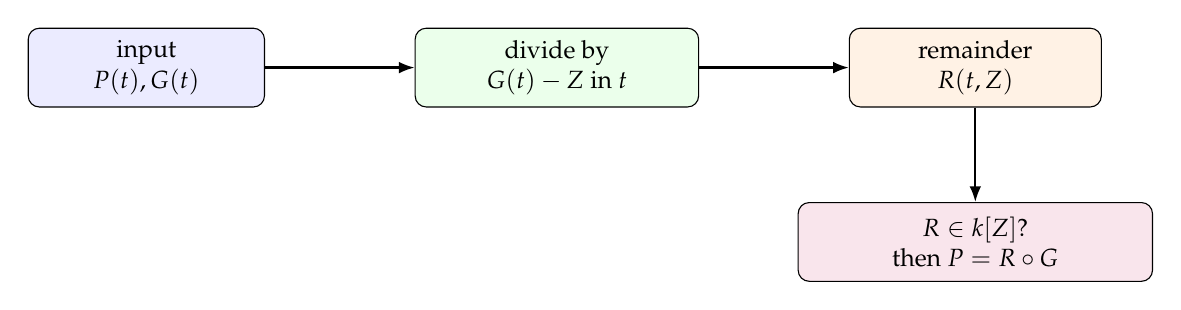
\begin{tikzpicture}[node distance=1.9cm, every node/.style={font=\small}]
    \node[draw, rounded corners, align=center, fill=blue!8, minimum width=3.0cm, minimum height=1.0cm] (input) {input\\\(P(t),G(t)\)};
    \node[draw, rounded corners, align=center, fill=green!8, right=of input, minimum width=3.6cm, minimum height=1.0cm] (divide) {divide by\\\(G(t)-Z\) in \(t\)};
    \node[draw, rounded corners, align=center, fill=orange!10, right=of divide, minimum width=3.2cm, minimum height=1.0cm] (rem) {remainder\\\(R(t,Z)\)};

    \draw[-{Latex[length=2mm]}, thick] (input) -- (divide);
    \draw[-{Latex[length=2mm]}, thick] (divide) -- (rem);

    \node[draw, rounded corners, align=center, fill=purple!10, below=1.2cm of rem, minimum width=4.5cm, minimum height=1.0cm] (decision) {\(R\in k[Z]\)?\\ then \(P=R\circ G\)};
    \draw[-{Latex[length=2mm]}, thick] (rem) -- (decision);
\end{tikzpicture}
\caption{Remainder extraction: the outer polynomial is the \(t\)-constant remainder after division by \(G(t)-Z\).}
\label{fig:algorithm}
\end{figure}

\section{Quotient-ring interpretation}

Let
\[
    A=k[x,y]/(f(x)-g(y)),
\]
and write bars for images in \(A\). In \(A\), the defining relation is
\[
    \ol{f(x)}=\ol{g(y)}.
\]
The theorem can be rephrased as the intersection identity
\[
    \ol{k[x]}\cap \ol{k[y]}
    =
    k[\ol{f(x)}]
    =
    k[\ol{g(y)}]
    \subseteq A.
\]
Indeed, if an element of \(\ol{k[x]}\cap \ol{k[y]}\) is represented both by \(p(x)\) and by \(q(y)\), then
\[
    p(x)-q(y)\in (f(x)-g(y)).
\]
By Theorem~\ref{thm:main}, there is \(s\in k[t]\) such that
\[
    p=s\circ f,
    \qquad
    q=s\circ g.
\]
Thus the common element is \(s(\ol{f(x)})=s(\ol{g(y)})\).

This quotient-ring perspective is often the cleanest conceptual summary: on the fiber product defined by
\[
    f(x)=g(y),
\]
any function depending only on \(x\) and also only on \(y\) must come from the shared base coordinate.

\section{Geometric reading}

Suppose, for intuition, that \(k\) is algebraically closed. The equation
\[
    f(x)=g(y)
\]
defines the fiber product of the maps
\[
    \A^1_x\longrightarrow \A^1,
    \qquad x\longmapsto f(x),
\]
and
\[
    \A^1_y\longrightarrow \A^1,
    \qquad y\longmapsto g(y).
\]
The divisibility condition
\[
    f(x)-g(y)\mid p(x)-q(y)
\]
means that the separated equation \(p(x)=q(y)\) holds scheme-theoretically on this fiber product. The theorem says that this can happen only for the tautological reason: \(p\) and \(q\) are obtained by applying the same polynomial \(s\) to the common base value.

\[
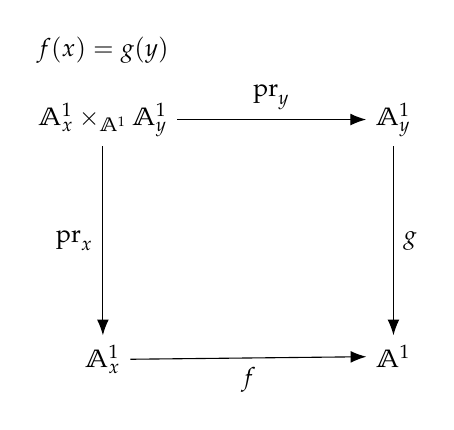
\begin{tikzpicture}[node distance=2.4cm, every node/.style={font=\small}]
    \node (PB) {\(\A^1_x\times_{\A^1}\A^1_y\)};
    \node (Y) [right=of PB] {\(\A^1_y\)};
    \node (X) [below=of PB] {\(\A^1_x\)};
    \node (B) [below=of Y] {\(\A^1\)};

    \draw[-{Latex[length=2mm]}] (PB) -- node[above] {\(\mathrm{pr}_y\)} (Y);
    \draw[-{Latex[length=2mm]}] (PB) -- node[left] {\(\mathrm{pr}_x\)} (X);
    \draw[-{Latex[length=2mm]}] (X) -- node[below] {\(f\)} (B);
    \draw[-{Latex[length=2mm]}] (Y) -- node[right] {\(g\)} (B);

    \node[above=0.25cm of PB] {\(f(x)=g(y)\)};
\end{tikzpicture}
\]

The diagram is only schematic: the algebraic proof does not require irreducibility of \(f(x)-g(y)\), separability of \(f\) or \(g\), or any assumption on the characteristic of \(k\).

\section{Application: a symmetric functional equation}

The criterion is particularly efficient when a functional equation says that a polynomial is constant on several algebraic branches lying above the same value of another polynomial. The following example is a model case.

\begin{proposition}[A three-branch symmetry]\label{prop:symmetric-functional-equation}
Assume \(\operatorname{char} k\neq 2\). Let \(\Phi(T)\in k[T]\). Let \(X\) be an indeterminate, and let \(\alpha,\beta\) be the two roots, in an algebraic closure of \(k(X)\), of
\[
    Y^2+XY+X^2+1=0.
\]
Equivalently, in square-root notation,
\[
    \alpha=\frac{-X+\sqrt{-3X^2-4}}{2},
    \qquad
    \beta=\frac{-X-\sqrt{-3X^2-4}}{2}.
\]
If
\[
    \Phi(\alpha)=\Phi(X)
    \qquad\text{and}\qquad
    \Phi(\beta)=\Phi(X)
\]
in the corresponding algebraic extension of \(k(X)\), then there exists \(h(T)\in k[T]\) such that
\[
    \Phi(T)=h(T^3+T).
\]
Conversely, every polynomial of the form \(h(T^3+T)\) satisfies these two branch identities.
\end{proposition}

\begin{proof}
Put
\[
    G(T)=T^3+T.
\]
A direct factorization gives
\[
    G(Y)-G(X)
    =
    (Y^3+Y)-(X^3+X)
    =
    (Y-X)(Y^2+XY+X^2+1).
\]
Thus \(Y=X\), \(Y=\alpha\), and \(Y=\beta\) are the three roots of
\[
    G(Y)-G(X)=0
\]
over an algebraic closure of \(k(X)\).

These three roots are distinct. The quadratic factor is separable because its discriminant is
\[
    X^2-4(X^2+1)=-3X^2-4,
\]
which is a nonzero element of \(k(X)\) when \(\operatorname{char} k\neq 2\). Also, \(Y-X\) and \(Y^2+XY+X^2+1\) are coprime in \(k(X)[Y]\), since substituting \(Y=X\) into the quadratic gives
\[
    3X^2+1,
\]
which is nonzero in \(k(X)\) in all characteristics, including characteristic \(3\), where it equals \(1\).

By hypothesis,
\[
    \Phi(\alpha)-\Phi(X)=0,
    \qquad
    \Phi(\beta)-\Phi(X)=0,
\]
and trivially
\[
    \Phi(X)-\Phi(X)=0.
\]
Therefore the polynomial
\[
    \Phi(Y)-\Phi(X)\in k[X,Y]
\]
vanishes at all three distinct roots of \(G(Y)-G(X)\), viewed as a polynomial in \(Y\) over \(k(X)\).

Since \(G(Y)-G(X)\) is monic of degree \(3\) in \(Y\), divide \(\Phi(Y)-\Phi(X)\) by \(G(Y)-G(X)\) in \(k[X][Y]\):
\[
    \Phi(Y)-\Phi(X)
    =
    Q(X,Y)(G(Y)-G(X))+R(X,Y),
    \qquad
    \deg_Y R<3.
\]
The remainder \(R\), considered in \(k(X)[Y]\), also vanishes at the three distinct roots of \(G(Y)-G(X)\). Since \(\deg_Y R<3\), it must be zero. Hence
\[
    G(Y)-G(X)
    \mid
    \Phi(Y)-\Phi(X)
    \qquad \text{in } k[X,Y].
\]
Equivalently,
\[
    G(X)-G(Y)
    \mid
    \Phi(X)-\Phi(Y).
\]
Applying Theorem~\ref{thm:main} with
\[
    f=g=G,
    \qquad
    p=q=\Phi,
\]
we obtain a polynomial \(h\in k[T]\) such that
\[
    \Phi(T)=h(G(T))=h(T^3+T).
\]

Conversely, if \(\Phi(T)=h(G(T))\), then whenever \(G(Y)=G(X)\), one has
\[
    \Phi(Y)=h(G(Y))=h(G(X))=\Phi(X).
\]
In particular, the identities hold for the two branches \(Y=\alpha\) and \(Y=\beta\).
\end{proof}

\begin{figure}[h]
\centering
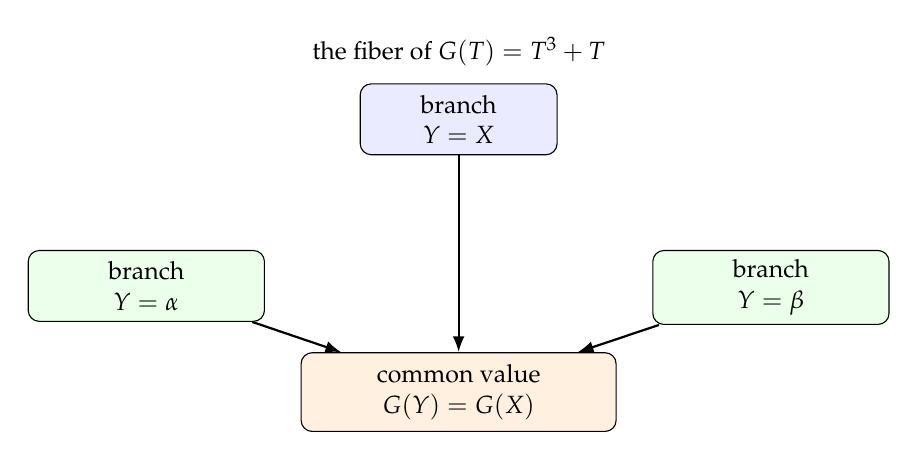
\begin{tikzpicture}[node distance=1.7cm, every node/.style={font=\small}]
    \node[draw, rounded corners, fill=blue!8, align=center, minimum width=2.5cm, minimum height=0.9cm] (x) {branch\\\(Y=X\)};
    \node[draw, rounded corners, fill=green!8, align=center, below left=of x, minimum width=3.0cm, minimum height=0.9cm] (a) {branch\\\(Y=\alpha\)};
    \node[draw, rounded corners, fill=green!8, align=center, below right=of x, minimum width=3.0cm, minimum height=0.9cm] (b) {branch\\\(Y=\beta\)};
    \node[draw, rounded corners, fill=orange!12, align=center, below=2.5cm of x, minimum width=4.0cm, minimum height=1.0cm] (base) {common value\\\(G(Y)=G(X)\)};

    \draw[-{Latex[length=2mm]}, thick] (x) -- (base);
    \draw[-{Latex[length=2mm]}, thick] (a) -- (base);
    \draw[-{Latex[length=2mm]}, thick] (b) -- (base);

    \node[above=0.1cm of x] {the fiber of \(G(T)=T^3+T\)};
\end{tikzpicture}
\caption{The two conjugate branches and the trivial branch lie in the same fiber of \(T^3+T\).}
\label{fig:branches}
\end{figure}

\begin{remark}
The word ``irreducible'' is not needed in the argument. The quadratic branch polynomial may or may not be irreducible over \(k(X)\), depending on the field. What matters is that the three branches are distinct over an algebraic closure of \(k(X)\). The main divisibility criterion itself does not require any separability hypothesis; separability only enters here because we infer divisibility from vanishing at distinct branches.
\end{remark}

\section{Fiber constancy in arbitrary characteristic}
\label{sec:fiber-multiplicity}

The preceding example uses distinct branches. For an arbitrary polynomial, the generic fiber can have multiplicities, and these must also be retained. The main theorem already handles them. The following consequence makes their role explicit without restricting the characteristic or assuming separability.

Let \(G\in k[T]\) be nonconstant. In characteristic zero put \(q=1\) and \(H=G\). In characteristic \(p>0\), let \(q=p^e\) be the largest power of \(p\) for which
\[
    G(T)=H(T^q),\qquad H\in k[T].
\]
Thus \(H'\ne0\). This decomposition simply groups the exponents of \(G\); it does not require taking roots of its coefficients. Let \(X\) be indeterminate and let \(\Omega\) be an algebraic closure of \(k(X)\).

For \(\Phi\in k[T]\), define its \emph{Hasse derivatives} by the polynomial identity
\[
    \Phi(T+U)=\sum_{j\ge0}\partial^{[j]}\Phi(T)\,U^j.
\]
In particular, \(\partial^{[0]}\Phi=\Phi\). These coefficients record vanishing to a prescribed order in every characteristic.

\begin{proposition}[Constancy with multiplicities]
\label{prop:fiber-multiplicity}
With the notation above, the following are equivalent:
\begin{enumerate}
    \item \(\Phi\in k[G]\).
    \item The classes of \(\Phi(Y)\) and \(\Phi(X)\) are equal in
    \[
        k[X,Y]/(G(Y)-G(X)).
    \]
    \item For every distinct root \(\alpha\in\Omega\) of \(G(Y)-G(X)\),
    \[
        \Phi(\alpha)=\Phi(X),\qquad
        \partial^{[j]}\Phi(\alpha)=0\quad(1\le j<q).
    \]
\end{enumerate}
Moreover, constancy on the geometric points alone has the exact characterization
\[
    \Phi(\alpha)=\Phi(X)\ \text{for every such }\alpha
    \quad\Longleftrightarrow\quad
    \Phi(T)^q\in k[G].
\]
\end{proposition}

\begin{proof}
First, \(H(Z)-G(X)\) has distinct roots over \(\Omega\). Indeed, a repeated root \(\beta\) would satisfy \(H'(\beta)=0\), making \(\beta\), and hence \(H(\beta)\), algebraic over \(k\). This contradicts \(H(\beta)=G(X)\), since \(G(X)\) is transcendental over \(k\).

For each root \(\beta\), the polynomial \(Y^q-\beta\) has a unique root \(\alpha\) in \(\Omega\) and equals \((Y-\alpha)^q\); this includes the case \(q=1\). Consequently, for some \(c\in k^\times\),
\[
    D(Y):=G(Y)-G(X)=c\prod_{\alpha}(Y-\alpha)^q,
\]
where the roots in the product are distinct. Thus every point of the generic fiber has exactly the same multiplicity \(q\).

Put \(E(Y)=\Phi(Y)-\Phi(X)\). Expanding \(E(\alpha+U)\), the Hasse derivative conditions in (3) say precisely that \((Y-\alpha)^q\mid E(Y)\). The factors for distinct \(\alpha\) are coprime, so (3) is equivalent to \(D\mid E\) in \(\Omega[Y]\).

This divisibility descends to \(k[X,Y]\) directly by polynomial division. The leading coefficient \(c\) of \(D\) lies in \(k^\times\), so division by \(D\) in \(k[X][Y]\) gives a remainder of \(Y\)-degree less than \(\deg G\). Divisibility over \(\Omega\) forces that same remainder to be zero. Hence (3) is equivalent to (2). Finally, the already proved Theorem~\ref{thm:main}, applied with \(f=g=G\) and \(p=q=\Phi\) in that theorem's notation, gives (2) if and only if (1). No assertion about branches was used in its free-module proof.

For the last assertion, pointwise constancy makes each \((Y-\alpha)\) divide \(E\), hence makes \(D\) divide \(E^q\). Since \(q\) is a power of the characteristic, or \(q=1\),
\[
    E(Y)^q=\Phi(Y)^q-\Phi(X)^q.
\]
The same division argument and Theorem~\ref{thm:main} give \(\Phi(T)^q\in k[G]\). Conversely, if \(\Phi(T)^q=S(G(T))\), then \(G(\alpha)=G(X)\) implies \(\Phi(\alpha)^q=\Phi(X)^q\). The map \(z\mapsto z^q\) is injective on the field \(\Omega\), so the values themselves agree.
\end{proof}

Condition (2) is constancy on the \emph{scheme-theoretic} fiber product: the quotient retains any nilpotents and therefore the multiplicities. When \(q=1\), no higher Hasse conditions are needed. In characteristic \(p>0\), the example \(G(T)=T^p\), \(\Phi(T)=T\) shows why pointwise constancy alone does not imply \(\Phi\in k[G]\), although \(\Phi^p\in k[G]\). More generally, \(G(T)=T^{p^e}\), \(\Phi(T)=T\) shows that the exponent \(q\) in the pointwise conclusion cannot uniformly be replaced by a smaller positive exponent. Ordinary derivatives cannot replace Hasse derivatives here: all positive-order ordinary derivatives of \(T^p\) vanish, but \(T^p\notin k[T^{p^2}]\).

\section{Why the nonconstancy hypotheses are necessary}

The assumptions \(\deg f>0\) and \(\deg g>0\) are essential.

\begin{example}
Let
\[
    f(t)=0,
    \qquad
    g(t)=t^2,
    \qquad
    p(t)=0,
    \qquad
    q(t)=t^3.
\]
Then
\[
    f(x)-g(y)=-y^2
\]
divides
\[
    p(x)-q(y)=-y^3
\]
in \(k[x,y]\). However, there is no polynomial \(s\in k[t]\) such that
\[
    q(t)=s(g(t))=s(t^2),
\]
because every polynomial in \(t^2\) is a linear combination of even powers of \(t\), whereas \(t^3\) is not.
\end{example}

\section{Some uses of the criterion}

The theorem is a useful algebraic test for recognizing common composition hidden inside a divisibility relation.

\begin{enumerate}
    \item \textbf{Composition detection.}
    If \(f(x)-g(y)\mid p(x)-q(y)\), then \(p\) lies in the subring \(k[f]\subseteq k[t]\), \(q\) lies in the subring \(k[g]\subseteq k[t]\), and the two factorizations use the same outer polynomial \(s\).

    \item \textbf{Fiber products of polynomial maps.}
    The quotient-ring identity
    \[
        \ol{k[x]}\cap \ol{k[y]}
        =
        k[\ol{f(x)}]
    \]
    says that the only functions on the fiber product \(f(x)=g(y)\) which separately come from the two factors are those descending from the base.

    \item \textbf{Separated-variable factorization.}
    Problems involving divisibility or factorization of polynomials of the form \(P(x)-Q(y)\) often reduce to understanding which one-variable polynomials are composite with a prescribed inner polynomial. The residue-rectangle method provides a direct coefficient comparison without needing irreducibility of \(f(x)-g(y)\).

    \item \textbf{Functional equations with conjugate branches.}
    Proposition~\ref{prop:fiber-multiplicity} gives an exact criterion over every field: constancy on the generic fiber, with its multiplicities retained, is equivalent to \(\Phi\in k[G]\). The multiplicities are measured by Hasse derivatives. Constancy on geometric points alone is equivalent to \(\Phi^q\in k[G]\), where \(q\) is the generic fiber's inseparable multiplicity. The cubic functional equation in Proposition~\ref{prop:symmetric-functional-equation} is the case \(q=1\).

    \item \textbf{Characteristic-free arguments.}
    The proof of Theorem~\ref{thm:main} uses only polynomial identities, freeness over subrings generated by nonconstant polynomials, and the diagonal specialization \(\U=\V\). It therefore works over arbitrary fields, including fields of positive characteristic.
\end{enumerate}

\section{Summary of the mechanism}

The proof has four moving parts.

\begin{enumerate}
    \item The one-variable decomposition
    \[
        k[x]=\bigoplus_{0\leq i<\deg f} k[f(x)]x^i
    \]
    records every polynomial uniquely by its residue degree modulo \(\deg f\).

    \item The two-variable decomposition
    \[
        k[x,y]
        =
        \bigoplus_{0\leq i<\deg f,\;0\leq j<\deg g}
        k[f(x),g(y)]x^i y^j
    \]
    gives a residue rectangle.

    \item In that rectangle, the identity
    \[
        (f(x)-g(y))H(x,y)=p(x)-q(y)
    \]
    becomes the coefficient system
    \[
        (\U-\V)C_{ij}(\U,\V)=\text{known coefficient}_{ij}.
    \]
    Setting \(\U=\V\) kills the factor \(\U-\V\), forcing all off-origin coefficients of \(p\) and \(q\) to vanish and forcing the origin coefficients to agree.

    \item Once the common composition is known, the outer polynomial is extracted by dividing \(P(t)\) by \(G(t)-Z\). The \(t\)-constant remainder is exactly the desired outer polynomial.
\end{enumerate}

Thus the divisibility condition is exactly equivalent to the existence of a common outer polynomial \(s\) with
\[
    p=s\circ f,
    \qquad
    q=s\circ g.
\]

\end{document}
